\documentclass[11pt, a4paper]{article}
\usepackage[english, science, titlepage]{ku-frontpage}
\usepackage[utf8]{inputenc}
\usepackage{booktabs}
\usepackage{amsfonts, amssymb}
\usepackage{mathtools}
\DeclarePairedDelimiter{\ceil}{\lceil}{\rceil}
\DeclarePairedDelimiter\floor{\lfloor}{\rfloor}

\usepackage{cite, hyperref, nameref}
\usepackage{natbib, apalike, url}

\usepackage{url}
\makeatletter
\g@addto@macro{\UrlBreaks}{\UrlOrds}
\makeatother

\setlength\arraycolsep{2 pt}
\setcounter{tocdepth}{2}
\setcounter{secnumdepth}{0}

\assignment{Master Thesis}
\author{Laura Perge}

\title{Time Series Classification with CNN:}
\subtitle{ Automated Trading by Pattern Recognition}
\date{Handed in: \today}
\advisor{Advisors: Rolf Poulsen, Kenneth H. M. Nielsen, Lasse Bøhling}
%\frontpageimage{example.png}

%% spellcheck-language "en"

\begin{document}
\maketitle

\tableofcontents

\begin{abstract}
    Something.
\end{abstract}

\section{Introduction}
People have been trading on financial markets for more than 200 years and with time, the internet, and technological advancement, the process has changed and evolved into what it is today:  
a versatile, international, online, easy-to-access, automated and truly immense beast. Its evolution is not over, however, and the mentioned features make it just the perfect subject of 
artificial intelligence and machine learning applications. 

But what were some major milestones of this evolution? As nicely summarized by \cite{rialtohistory}  employing algorithms in trading for calculation of asset prices goes back to the beginning of the 20th century. In the early 1950s, Harry Markowitz brought computational finance to existence in the pursuit of portfolio optimization. During that time, the computational 
resources were inadequate to efficiently utilize these algorithms in trading. From the 1970s to 1990s, 
large-scale computerization, the introduction of PCs, the internet and then amongst other systems the ECN (Electronic Communication Network) completely changed the game. Automation became a 
feasible solution, and algorithms are way faster to react with Buy/Sell orders on the market than humans. Trading is now not only for institutions or professionals and a chosen few but for 
every person with access to the internet. Intraday and high-frequency trading emerged and so, using algorithmic trading strategies with automated execution has become crucial in order to 
trade on these markets. 

There is another influential idea that has been around for several decades but has just gained space due to technological progress and the wide-spread access to computational power: artificial intelligence, more 
concisely machine learning and deep learning. 
The first paper about creating a model of the human neural networks was by \cite{mcculloch1943logical} and many more have followed ever since. 
One more achievement related to our topic was the first convolutional neural network (CNN) by \cite{fukushima1979neural} which is the first deep learning model for handwritten character and other 
pattern recognition.

CNN is an exceptionally popular tool nowadays, especially, in the field of image recognition. We recount the details and reasons behind this in the section \nameref{sec:DM}.
The reasons to apply CNN for our problem is supported by both a bottom-up and top-down way. The top-down comes from the recently mentioned recognition of the technique which 
means plenty of resources, established and accurate models together with the ability of feature extraction which comes in handy for time series pattern recognition tasks. 
The bottom-up approach arises naturally from the idea of turning time series into images and label them, so these labels can be assigned to the new images later which, essentially, is 
just an image classification task. 

Generally, when we search for ways of making money by trading on financial markets, the common approach appears to be forecasting time series adopting either a more traditional or a cutting-edge technique. 
Traditional means include autoregressive (AR) and/or moving average models (MA, ARMA) which are limited by the assumed linear relationship between the present and previous values of the univariate time series in question. 
Another limitation is the expectation of stationarity which is solved in the ARIMA (autoregressive integrated moving average) model that still remains linear but takes some preliminary transformation steps 
to turn the problem into a stationary ARMA. Although linearity is mostly acceptable in time series prediction problems, it is not true in all cases, and for that reason  
ARCH and GARCH (\textit{generalized} autoregressive conditional heteroskedasticity) models were invented. These complex models provided solutions to time series analytics which have long been in use and provide explicit insight into the time-dependence structure of the data.\footnote{The interested reader can find more information on these methods in for example Section 2 and 3 of \cite{tsay2005analysis}.}
In the field of AI and deep learning, recurrent neural networks (RNN) is a kind that was engineered to deal with sequential data. To address the issue of remembering long term temporal dependencies long 
short term memory (LSTM) networks were created which are heavily used in time series forecasting problems (\cite{Hochr97LSTM}). 
However, there are plenty of difficulties when it comes to prediction of financial time series. Accurate forecasting with these techniques require a lot of data, moreover, financial time series are many times non-stationary and influenced by regime changes \cite{lemus_2018}.

On the other hand, in this paper, we avert from the application of forecasting the next element of a series and concentrate on predicting trading decisions based on the present prices. We train the model to recognize periods, in the end of which one should make a buying or selling order. 

\textbf{OBJECTIVES: TO BE MODIFIED ACCORDING TO OUTCOME}
The goal of this paper is to develop a simple but powerful model that can make real-time trading decisions utilizing a convolutional neural network. For this, we need to capture as much dynamic 
and static information from the one-dimensional time series as possible which we achieve by turning them into images. The classification exercise requires labels which we choose to represent trading orders of "Buy", "Sell" and "Hold". 
These are preliminarily defined on the training set using a suitable algorithm that is designed to ensure profitability. The ultimate objective is a compact multilevel trading model that takes care of both the creation of image representations and the prediction of financially successful trading strategies using these images, for data that is fed to the model in real time. We also make a contrast between a model trained and used for a specific financial instrument and a "universal" model of multiple assets motivated by the work of \cite{sirignano2018universal}. The expected outcome is that the universal model will give more robustly successful results.

In the section \nameref{sec:RelWork}, we look at the path of publications that motivated and built the foundation of our approach. Then, the section \nameref{sec:DM} provides us with information about the kind of data we use throughout 
the paper, moreover, we introduce the methodologies implemented from the data preparation to the prediction phase. These include the transformation of one-dimensional time series into two-dimensional images, 
how we proceed to create appropriate labels for these images, how we construct and train our CNN model on them and return predictions using the model. 
Afterward, in \nameref{sec:ER} we examine the results and present them in a three-fold manner:
technical fitness (how accurate is the classification?), financial profitability (how high are the returns?), swiftness (how quick is the model to come up with a prediction?). In the section \nameref{sec:Discuss}, an assessment of the presented results is carried out.
The last section is the \nameref{sec:Conclusion} which judges how much 
we closed in on grasping our objectives and what are some possible proceedings of this work.

\section{Related Work}
\label{sec:RelWork}

The overall heuristics of this paper largely resembles the one published by \cite{sezer2018algorithmic}. They propose a deep CNN based algorithmic trading model which they train on financial time series to predict trading orders. The paper diverts from our approach in that it transforms the one dimensional time series into images using 15 different technical indicators over different time periods and fits them into a grid. Their results showed that the performance of their model was quite good against Buy \& Hold and other algorithmic methods even on periods long out of sample. Their conclusion states that they could potentially improve performance by creating more meaningful images.

One potential issue with the image transformation methodology used by the mentioned paper is that the resulting plot does not directly represent the input time series. The image is dependent of the choice of technical indicators and their ordering in the grid. Therefore, we turn to \cite{hatami2018classification} which proposes a similar model but with using Recurrence Plots for transformation; and \cite{wang2015encoding} which uses Markov Transition Fields and Gramian Angular Fields in the different color channels (RGB) of the resulting image. Both methods require a window of elements from the series and maps those to two dimensions according to different formulas which we cover in details in the section \nameref{subsec:DM:TS2IM}.

\section{Data and Methodology}
Overall, 6 models are trained, tuned and tested. There are 5 individual models each exclusively trained and tested on one assigned dataset. This is used to analyze the performance of asset-specific model builds. 
Then, we train the universal model on data coming from 35 financial assets, including the 5 used in the asset-specific models, and test it on these 5 assets once again. This system allows us to compare the performance of the universal model to the asset-specific ones.

In a real life scenario, the asset-specific models translate to a trader picking certain assets to trade, then gathering all available historical prices for those assets, training and tuning a model for each of them and then use one model per asset to generate trading signals. 
On the other hand, we could imagine a trader gathering data of many assets, including those he wishes to trade, train and tune one universal model on all available data, and use that to generate trading signals for any of the instruments selected for trading. Also, in the second case the trader can start generating trading signals for each of the assets used for training the universal model while in the asset-specific case he needs to collect the historical data of the new asset and build a new model for it.

In the upcoming subsections we will look into what data is used for each of the 6 models, how training, tuning and testing is approached to get comprehensive results, and what other trading techniques we match our performance against.

\label{sec:DM}
\subsection{Data}
\label{subsec:DM:Data}

The 5 asset-specific models are based on the historical adjusted daily closing prices of the following indices, stocks, and ETF:

\begin{itemize}
    \item S\&P 500,
    \item Nikkei 225,
    \item Nasdaq Composite,
    \item Apple Inc.,
    \item SPDR S\&P 500 ETF Trust.
\end{itemize} 

The universal model contains all five assets above and others listed in table \ref{tbl:univ_data}. The assets are selected to represent various asset classes: major stocks, stock indices, exchange traded funds, foreign exchange rates and commodity prices.

\begin{table}[]
\begin{tabular}{@{}lll@{}}
\toprule
\textbf{Name}                   & \textbf{Symbol} & \textbf{Dates}          \\ \midrule
\textbf{Main assets}            &                 &                         \\
S\&P500                         & GSPC            & 1950/01/03 - 2019/06/07 \\
Nikkei225                       & N225            & 1965/01/25 - 2019/06/07 \\
Nasdaq                          & IXIC            & 1971/02/05 - 2019/06/07 \\
AAPL                            & AAPL            & 1980/12/12 - 2019/06/07 \\
SPY                             & SPY             & 1993/01/29 - 2019/06/07 \\ \midrule
\textbf{Stock Indices}          &                 &                         \\
DJI                             & DJI             & 1985/01/29 - 2019/06/07 \\
DAX30                           & GDAXI           & 1987/12/30 - 2019/06/07 \\
Shanghai Composite              & SSI             & 1990/12/19 - 2019/06/07 \\
VIX                             & VIX             & 1990/01/02 - 2019/06/05 \\
FTSE100                         & INDEXFTSE: UKX  & 1997/10/20 - 2019/05/31 \\
FTSE250                         & INDEXFTSE: MCX  & 1997/10/20 - 2019/05/31 \\
FTSE350                         & INDEXFTSE: NMX  & 1997/10/20 - 2019/05/31 \\
Eurostoxx 50                    & STOXX50E        & 1986/12/31 - 2019/06/07 \\
Russell 2000                    & RUT             & 1987/09/10 - 2019/06/07 \\ \midrule
\textbf{Exchange Traded Funds}  &                 &                         \\
QQQ                             & QQQ             & 1999/03/10 - 2019/06/07 \\
XLF                             & XLF             & 1998/12/22 - 2019/06/07 \\
XLU                             & XLU             & 1998/12/22 - 2019/06/07 \\
XLP                             & XLP             & 1998/12/22 - 2019/06/07 \\
EWZ                             & EWZ             & 2000/07/14 - 2019/06/07 \\
EWH                             & EWH             & 1996/04/01 - 2019/06/07 \\
XLY                             & XLY             & 1998/12/22 - 2019/06/07 \\
XLE                             & XLE             & 1998/12/22 - 2019/06/07 \\ \midrule
\textbf{Foreign Exchange Rates} &                 &                         \\
GBPUSD                          & DEXUSUK         & 1971/01/04 - 2019/05/31 \\
AUDUSD                          & DEXUSAL         & 1975/01/02 - 2019/05/31 \\
NZDUSD                          & DEXUSNZ         & 1971/01/04 - 2019/05/31 \\
EURUSD                          & DEXUSEU         & 1999/01/04 - 2019/05/31 \\ \midrule
\textbf{Commodities}            &                 &                         \\
Copper                          & Copper          & 1959/07/06 - 2019/06/07 \\
WTI                             & DCOILWTICO      & 1986/01/02 - 2019/06/03 \\
Europe Brent Spot Price         & FOB             & 1987/05/20 - 2019/06/03 \\
Gold                            & XAUUSD          & 1979/12/29 - 2019/06/07 \\
Silver                          & XAGUSD          & 1982/07/02 - 2019/06/07 \\
Platinum                        & Platinum        & 1969/01/02 - 2019/06/07 \\
Corn                            & Corn            & 1959/07/01 - 2019/06/07 \\
Coffee                          & Coffee          & 1973/08/20 - 2019/06/07 \\
Soybean oil                     & Soybean oil     & 1960/10/26 - 2019/06/07
\end{tabular}
\caption{Overview of datasets. The main assets' daily adjusted closing prices are each individually used to train and test asset-specific models, while all of the 35 assets' daily (adjusted) closing prices are used to train the universal model. }
\label{tbl:univ_data}
\end{table}

\textbf{DO I HAVE TO STATE SOURCES? IF I DO, IS IT ENOUGH TO PRESENT A MORE DETAILED TABLE IN THE APPENDICES WITH LINKS AND DATES OF DOWNLOAD?}

Each asset's time series take values on business days. One-off missing values are imputed using forward filling which is just propagating the last valid non-missing value to the gaps. Afterwards, each price series is turned into return series. The return $r$ at time $t$ is defined $r_t = \frac{p_t}{p_{t-1}}-1$ where $p_t$ is the price given at any time point $t$.

In terms of scaling, Recurrence Plots and Markov Transition Fields require no scaling steps, while for the Gramian Angular Field transformation, we first use min-max normalization between $[-1, 1]$ according to the general formula for $[a, b]$
\begin{equation}
\label{eq:minmax}
    x^{scaled}_i =(b-a)\frac{x_i-\min(x)}{\max(x) - \min(x)} + a
\end{equation}
given $x = (x_1, \dots, x_n)$ is a univariate time series and $x_i$ is its $i^{th}$ element. Note, that the scaling is done separately on the testing and training data to avoid look-ahead bias.

\subsection{Transformation Strategies: Time Series to Images}
\label{subsec:DM:TS2IM}

We cover the three techniques mentioned before: Recurrence Plots, Markov Transition Fields and Gramian Angular Fields. All three methods are applied on sliding windows of size $s = 20$ (\textbf{TBM!!}) of the different return time series. This means that for $n$ return values we get $(n - s + 1)$ images. 

The \textbf{Recurrence Plots (RP)} originally introduced by \cite{jp1987recurrence} implemented according to \cite{hatami2018classification} are useful when we wish to represent the periodicity of trajectories going through a phase space. The issue with visualization that the RP solves appears when the phase space has more than three dimensions. A recurrence represents the time a trajectory gets back to a previously visited location. In Figure \ref{fig:RP_Def} we use the same explanation presented in Figure 1 of \cite{hatami2018classification}. In the plots it can be observed, how certain values tend to follow each other, for example $x_3 = 1, x_4 = 3$ and then this pattern re-occurs at $x_6, x_7$ which is reflected by $s_3$ and $s_6$ falling to the same phase on the map, and thus by the pixel at $(s_3, s_6)$ being equal to zero.

\begin{figure}[ht]
    \centering
    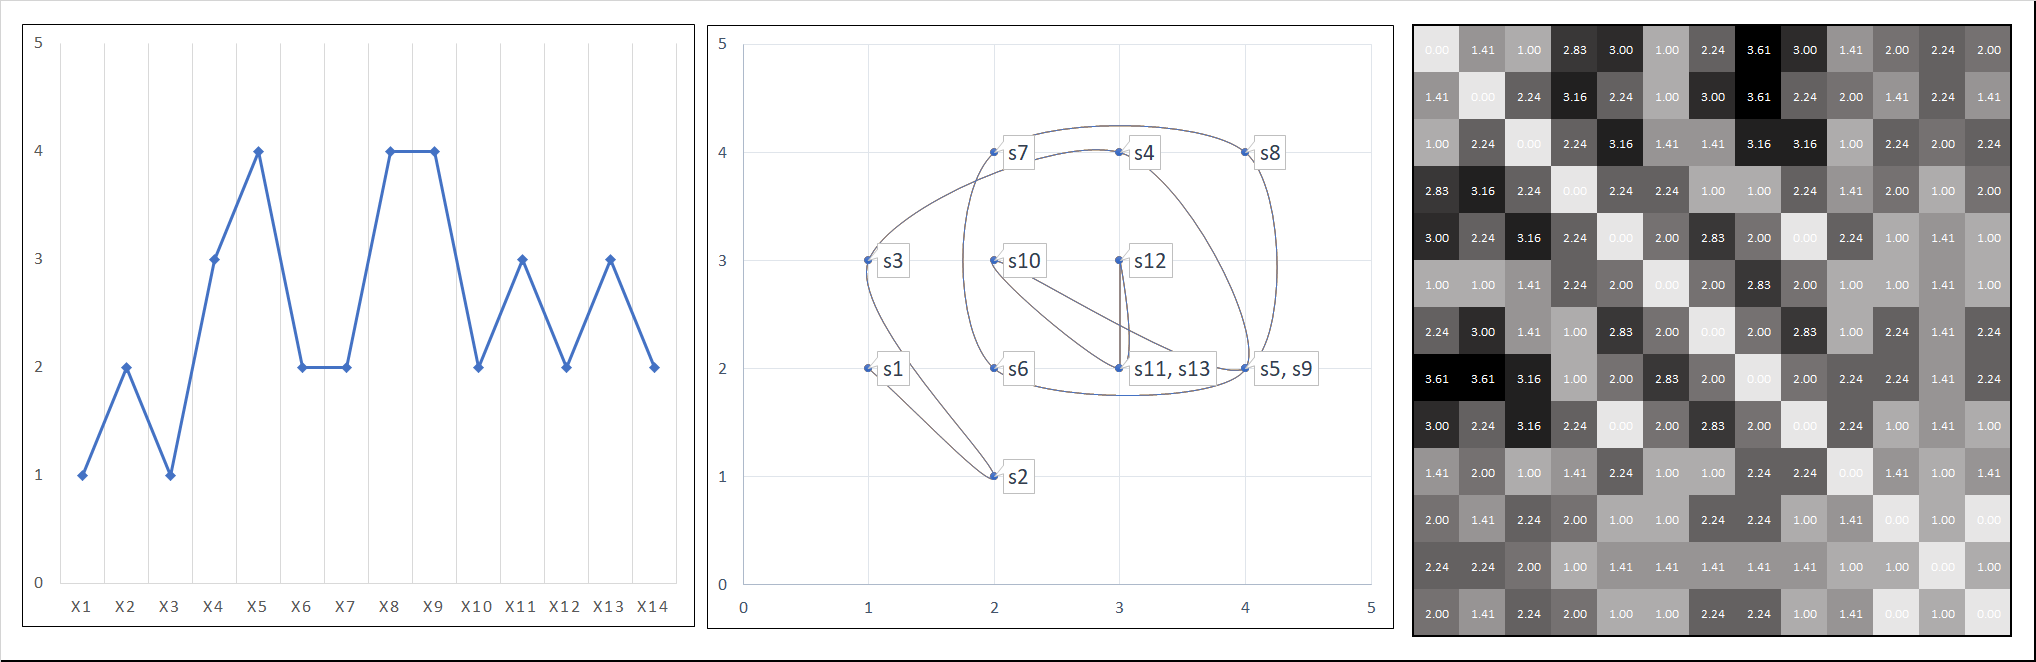
\includegraphics[width=\textwidth]{images/RP.PNG}
    \caption{The left plot shows a time series of 7 observations $x_t$, $t=1,\dots,7$. The plot in the middle shows the two dimensional phase space trajectory that is created from $x$ using a time delay of $\tau = 1$. The states are denoted by $s_k$ for $k=1,\dots,13$ where $s_k = (x_k, x_{k+1})$. On the right, the recurrence plot is a matrix of Euclidean distances between the 6 states: $R_{i,j} = Euclidean(s_i,s_j)$.}
    \label{fig:RP_Def}
\end{figure}

After the recurrence plots are created, we scale them to fall in the interval $[0, 1]$ using the appropriate min-max scaling introduced in Equation \ref{eq:minmax} which is a requirement of the CNN input. 

As it is pointed out in \cite{hatami2018classification}, time series tend to show recurrent behaviour like periodicity, and this phenomenon is generally present in dynamic nonlinear systems or stochastic processes that generate the series. The recurrence plot, as described previously via Figure \ref{fig:RP_Def}, reveals which are the phases that trajectories tend to return to. To attain such a plot, each element of it is the result of this formula:
\begin{equation}
\label{eq:RP_R}
    R_{i,j} = \theta(\epsilon-||\vec{s}_i - \vec{s}_j||),\quad \vec{s}(.) \in \mathbb{R}^m, \quad i,j = 1,\dots,K
\end{equation}
where K is the number of considered states $\vec{s}$, $\epsilon$ is a threshold distance, $||.||$ a norm (Euclidean in our case), and $\theta(.)$ the Heaviside function\footnote{The Heaviside function is defined as: $\theta(x) = \frac{d}{dx}\max(0,x)$ for $x \neq 0$}. Summing up the process of creating a recurrence plot for our purposes: first, we start out with a window containing $20$ consequent return values of an asset; then we create the two-dimensional phase space trajectory ($m=2$) from these series which results in $19$ states; finally, the R-matrix is calculated based on Equation \ref{eq:RP_R} but with a small change. The formula, due to the $\epsilon$ threshold parameter, would give us a matrix of ones and zeros, and to avoid this information loss we simply skip this step and work with the resulting grey-scale images. Also, we use min-max scaling on each resulting image of $(19 \times 19)$ to $[0, 1]$ in order to satisfy the requirements of the CNN's input vectors. Afterwards, to fit the image size of the two other transformation strategies introduced later, we add a size $1$ zero-padding to the right and bottom of the image.

% potentially mention RP on prices that increase or decrease similar while on returns it is more distinctive

Another image transformation used is the \textbf{Gramian Angular Field (GAF)} that translates the typical Cartesian coordinates into a polar coordinate system. The technique is introduced in \cite{wang2015encoding}, and is based on the Gramian matrix (named after J{\o}rgen Pedersen Gram), the entries of which are given by $G_{ij} = \langle v_i,v_j \rangle$ for a set of vectors $v_1,\dots, v_n$. These entries are inner products which measure the "similarity" of the two vectors. The Gram matrix is generally used for the calculation of the linear independence of a set of vectors. A beneficial property of the Gram matrix is that it preserves temporal dependency in the geometrical setting of the matrix, time flows from the top left to the bottom-right. For example, the Gramian matrix of a univariate time series: $x_t$ for $t=1, 2, 3$ can be computed as:

$$
G =\begin{pmatrix} 
\langle x_1,x_1 \rangle & \langle x_1,x_2 \rangle & \langle x_1,x_3 \rangle \\
\langle x_2,x_1 \rangle & \langle x_2,x_2 \rangle & \langle x_2,x_3 \rangle \\
\langle x_3,x_1 \rangle & \langle x_3,x_2 \rangle & \langle x_3,x_3 \rangle \\
\end{pmatrix}
$$

As noted in \cite{gaf_medium} the use of the Gramian matrix can be motivated by the fact that plain univariate time series prove unsuccessful in explaining co-occurence and latent states in the data and the Gramian matrix provides an alternative visualization. This same article also shows that the traditional Gram matrix is unsuccessful in making a distinction between the Gaussian noise and the valuable information in the data, thus the entries of the GAF matrix are not simply given by the inner product (in an Euclidean setting). Following the definition in \cite{wang2015encoding}, to create a GAF plot from a time series $X = \{x_1,x_2, \dots x_n\}$ of n valued real observations, we first rescale $X$ using min-max scaling to the $[-1,1]$ interval, as described previously in Equation \ref{eq:minmax}, and end-up with the scaled series $\Tilde{X}$. Now, we transform the time series into polar coordinates:
\begin{align}
\label{eq:gafencode}
    \begin{cases}
        \phi_i = \arccos(\Tilde{x}_i), \quad -1 \leq \Tilde{x}_i \leq 1, \quad \Tilde{x}_i \in \Tilde{X}\\
        r_i = \frac{t_i}{N}, \quad t_i \in \mathbb{N}
    \end{cases}
\end{align}
i.e. we convert the timestamp $t_i$ dividing by $N$ (the number of series instances) and get the radius. As for the angles, they are the angular cosine of the scaled series. Then, we create the Gramian Angular Field by taking the cosine sum between each pair of angles:

\begin{equation}
\label{eq:GAF}
    GAF =\begin{pmatrix} 
\cos(\phi_1 + \phi_1) & \cdots & \cos(\phi_1 + \phi_n)\\
\cos(\phi_2 + \phi_1) & \cdots & \cos(\phi_2 + \phi_n)\\
\vdots & \ddots & \vdots\\
\cos(\phi_n + \phi_1) & \dots & \cos(\phi_n + \phi_n)\\
\end{pmatrix} \\
= \Tilde{X}' \cdot \Tilde{X} - \sqrt{I-\Tilde{X}^2}' \cdot \sqrt{I-\Tilde{X}^2}
\end{equation}
where $I$ is the unit row vector $[1, 1, \dots, 1]$. Notice, that this is a Gramian-like matrix with a penalized inner product given by\footnote{Please see Appendices \nameref{app:GAF} for the proof.}: $\langle x, y\rangle - \sqrt{1-x^2} \cdot \sqrt{1-y^2}= x \cdot y - \sqrt{1-x^2} \cdot \sqrt{1-y^2}$. There are several advantages to this construction one of which is preserving the absolute temporal relations. Another aspect is that the diagonal sustains the original (although transformed) time series. Furthermore, the entries $GAF_{ij}$ of the matrix represent the temporal correlation (cosine-similarity) with respect to the different $k= |i-j|$ time intervals, and the main diagonal displays the case of $k=0$. Figure \ref{fig:GAF} shows how the transformation happens for an example scaled time series of $14$ observations. Time can again be tracked going from the top-left to the bottom-right corner.

\begin{figure}[ht]
    \centering
    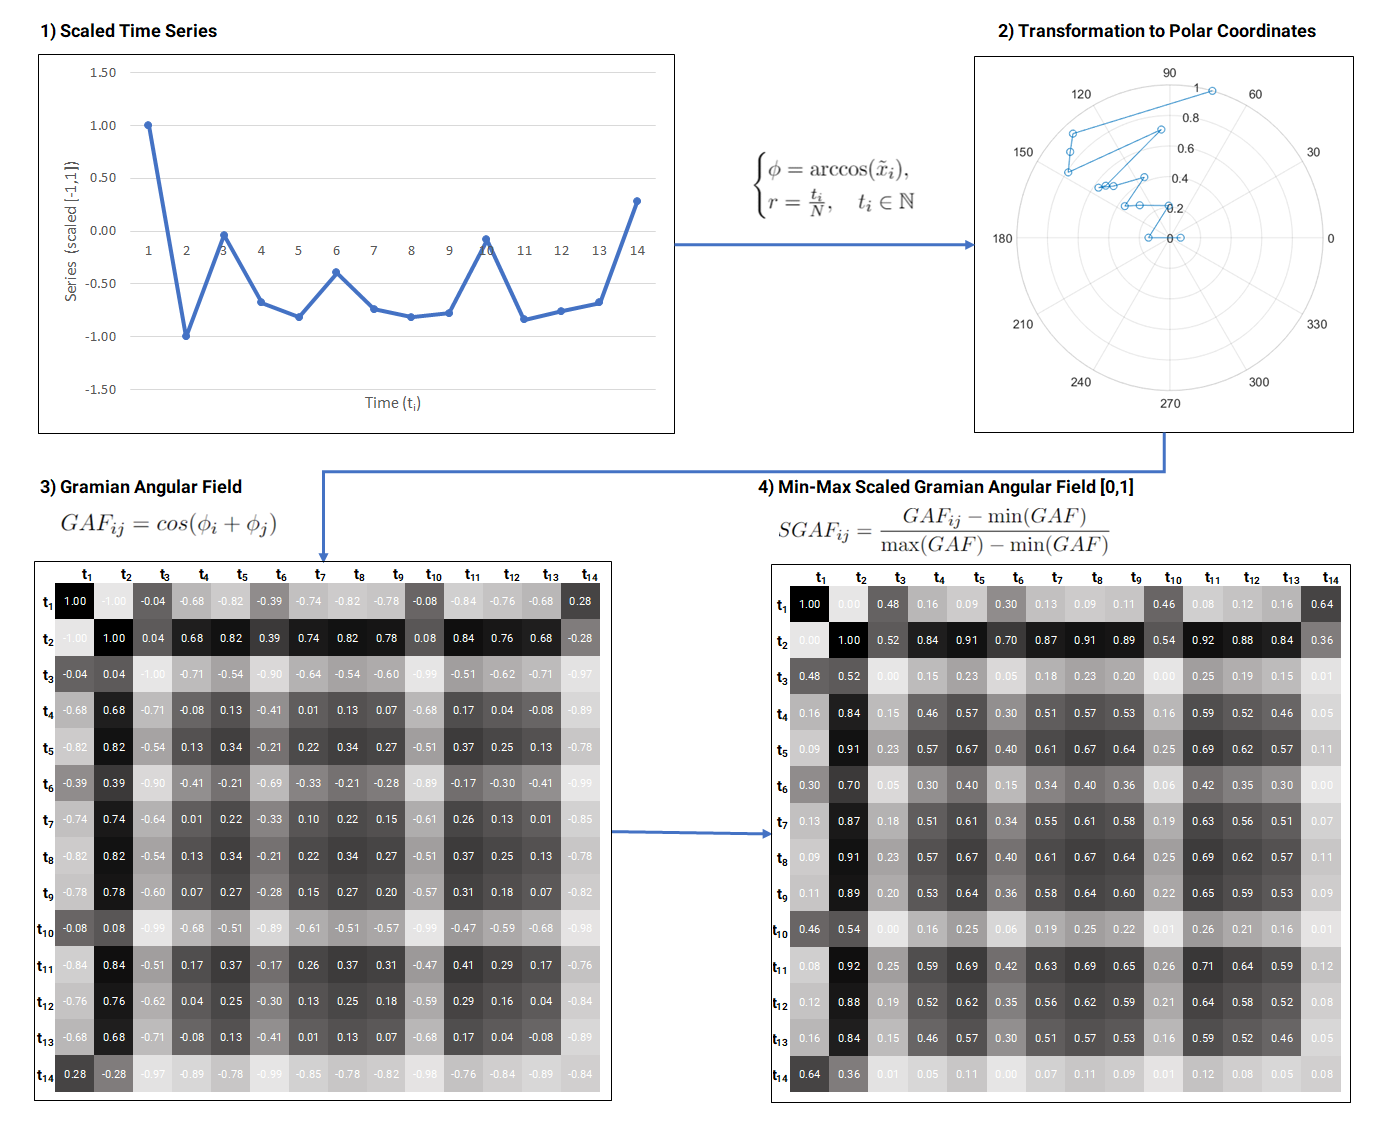
\includegraphics[width=\textwidth]{images/GAF.png}
    \caption{Plot 1 shows the time series scaled to the interval [-1, 1] which is then transformed to polar coordinates. In the polar coordinate system in Plot 2, the first point is the closest to the center, then as time moves forward, the coordinates vary among different angles but move further and further out towards the boundaries of the unit circle. Plot 3 shows the GAF plot that we get by applying the formula in Equation \ref{eq:GAF}. Before applying the CNN, we use min-max scaling to the interval $[0,1]$ to fit the expected input of the model. As Plot 4 demonstrates, this scaling does not change the appearance of the image.}
    \label{fig:GAF}
\end{figure}

% Importantly, the described encoding map in Equation \ref{eq:gafencode} is bijective as $cos(\phi)$ is monotonic given that $\phi \in [0, \pi]$ which IS NOT TRUE HERE, is it? for the single angles yes, but we add them up, which results in non-bijective transformation, for the different input we can get the same output, maybe the radius makes it?

The third and last transformation strategy introduced is called \textbf{Markov Transition Field (MTF)} and it entails encoding dynamic transition probabilities from a Markov Transition Matrix of discretized quantile bins in a quasi-Gramian matrix. The algorithm is introduced in \cite{wang2015encoding} and inspired by \cite{campanharo2011duality}.

In its essence, the method consists of encoding the dynamic transition probabilities in a Markov Transition Matrix and then from that matrix create a new one that also preserves information about the sequentiality of the time series which is the MTF.
To be more precise, given a time series $X_t$ (which, in our case, is the return series) we first identify its $Q$ quantile bins $q_j$ $(j \in [1,Q])$. In Figure \ref{fig:MTF}, Plot 1 illustrates this step. Afterwards, matrix $V$ is a $Q \times Q$ weighted adjacency matrix, with $V_{ij}$ representing the count of transitions from $q_i$ to $q_j$ within one time step. 
%This is also a first-order Markov chain along the time axis.
Then, the Markov Transition Matrix denoted by $W$ is constructed by normalization of $V$:

\begin{equation}
\label{eq:W}
    W_{ij} = V_{ij}/\sum_j V_{ij}.
\end{equation}

Thus, $W_{ij}$ gives us the probability of moving from the $i^{th}$ bin to the $j^{th}$ bin within one time step. Now, the issue with this matrix is that we lose a lot of information and it fails to represent that the data is serial in time. Therefore, \cite{wang2015encoding} suggests a design that sustains the time dependence via the locations of the values in the matrix. The Markov Transition Field can then be described as:

\begin{equation}
    \label{eq:MTF}
        MTF =\begin{pmatrix} 
    W_{ij|x_1 \in q_i, x_1 \in q_j} & \cdots & W_{ij|x_1 \in q_i, x_n \in q_j}\\
    W_{ij|x_2 \in q_i, x_1 \in q_j} & \cdots & W_{ij|x_2 \in q_i, x_n \in q_j}\\
    \vdots & \ddots & \vdots\\
    W_{ij|x_n \in q_i, x_1 \in q_j} & \dots & W_{ij|x_n \in q_i, x_n \in q_j}
    \end{pmatrix}
\end{equation}
and an example can be observed in Plot 3 of Figure \ref{fig:MTF}. This resulting image, similarly to the previous two representations trails the flow of time from the top-left to the bottom-right corner.
The entries of this matrix are already in the range $[0,1]$, so there is no need for further scaling before feeding it to the CNN. The images are created with the same sliding window technique discussed previously. A parameter to decide on is the number of quantile bins to create, and with window size set to $20$ it is set to $5$ (TBD!!!!) in our image construction.\footnote{It should be noted that the number of bins can be optimized via costly hyperparameter optimization but due to limitations in time and computational power this was not carried out in the study.}
The MTF can also be understood as the multispan transition probabilities of the series within one step at different points in time.

\begin{figure}[ht!]
    \centering
    
\includegraphics[width=\textwidth]{images/MTF.png}
    \caption{Plot 1 shows the time series which is assigned to $Q=4$ quantile bins. In Plot 2.a), we can inspect th preliminary state of the Markov Transition Matrix $V$, the elements of which are the counts of the different transitions in the time series $X$, and in Plot 2.b) $W$ is the so-called right stochastic matrix or Markov Transition Matrix, a real stochastic matrix with transition probabilities between the different bins and each row summing to $1$ (see Equation \ref{eq:W}). Plot 3 shows the MTF plot that we get by applying the formula in Equation \ref{eq:MTF}.}
    \label{fig:MTF}
\end{figure}

\subsection{Image Labelling}
\label{subsec:DM:IL}
The image labelling is done in two steps. First, we label the original time series and, in a second step, the images using the labels from Step 1.
The labelling algorithm is based on a simple idea and follows the one applied in \textit{Algorithm 1 in} \cite{sezer2018algorithmic}.

The algorithm for the time series is as follows. We choose an odd labelling window size $l = 3$. The oddness is required since we slide this labelling window along the series and label the middle element of the window as "Buy" ("Sell") if the mid point of the window is the minimum (maximum) of the values in the window, otherwise they are "Hold". The process is illustrated in Plots 1-6 in Figure \ref{fig:Labelling}. 
Two special cases are when, after a plunge, the series remains constant and then goes up again, and vice versa. They are also shown in Plots 7-10 in Figure \ref{fig:Labelling}, and the rule is as follows: 
given the middle observation in the labelling window is sharing its property of being a local minimum (maximum) with at least one of its direct neighbours, then the label is a "Buy" ("Sell") only if the observation following the mid point is strictly greater (strictly less) than the mid point.

In Step 2, we digress from the mentioned literature. Each image is labelled as the last element of the series that is used for creating the image. In other words, considering image window size of $s$ and return series $X_t$ for $t = 1, \dots, n$ for $n > s$ which has labels defined by\footnote{The notation $\lfloor \cdot \rfloor$ refers to the floor function.} 
$L_{\bar{t}}$ for 
$\bar{t} = \left(1+\lfloor \frac{l}{2} \rfloor\right), \dots, \left(n-\lfloor \frac{l}{2} \rfloor\right)$ with labelling window size $l$, and each image made up of the subset of the series given by
$X_{(i,\dots,(i+s-1))}$  
for every
$i = \left(1+\lfloor \frac{l}{2} \rfloor\right), \dots, \left(n-s+1-\lfloor \frac{l}{2} \rfloor\right)$ gets the label $L_{i+s-1}$. All in all, this indicates that given a series of $n$ returns, we can label $\left((n - s + 1)-\lfloor \frac{l}{2} \rfloor\right)$ of the $(n - s + 1)$ images created.
There are multiple reasons to pursue this approach. Firstly, if we were to label an image based on the price at its mid point, the prediction of a label would come too late to actually trade at that price. Secondly, the choice of the labelling window size does not have to match the window size used for image creation which is also beneficial because the labelling window size allows us, to some extent, to choose the frequency of "Buy" and "Sell" orders because a smaller window size identifies more of them. 

\begin{figure}[ht]
    \centering
    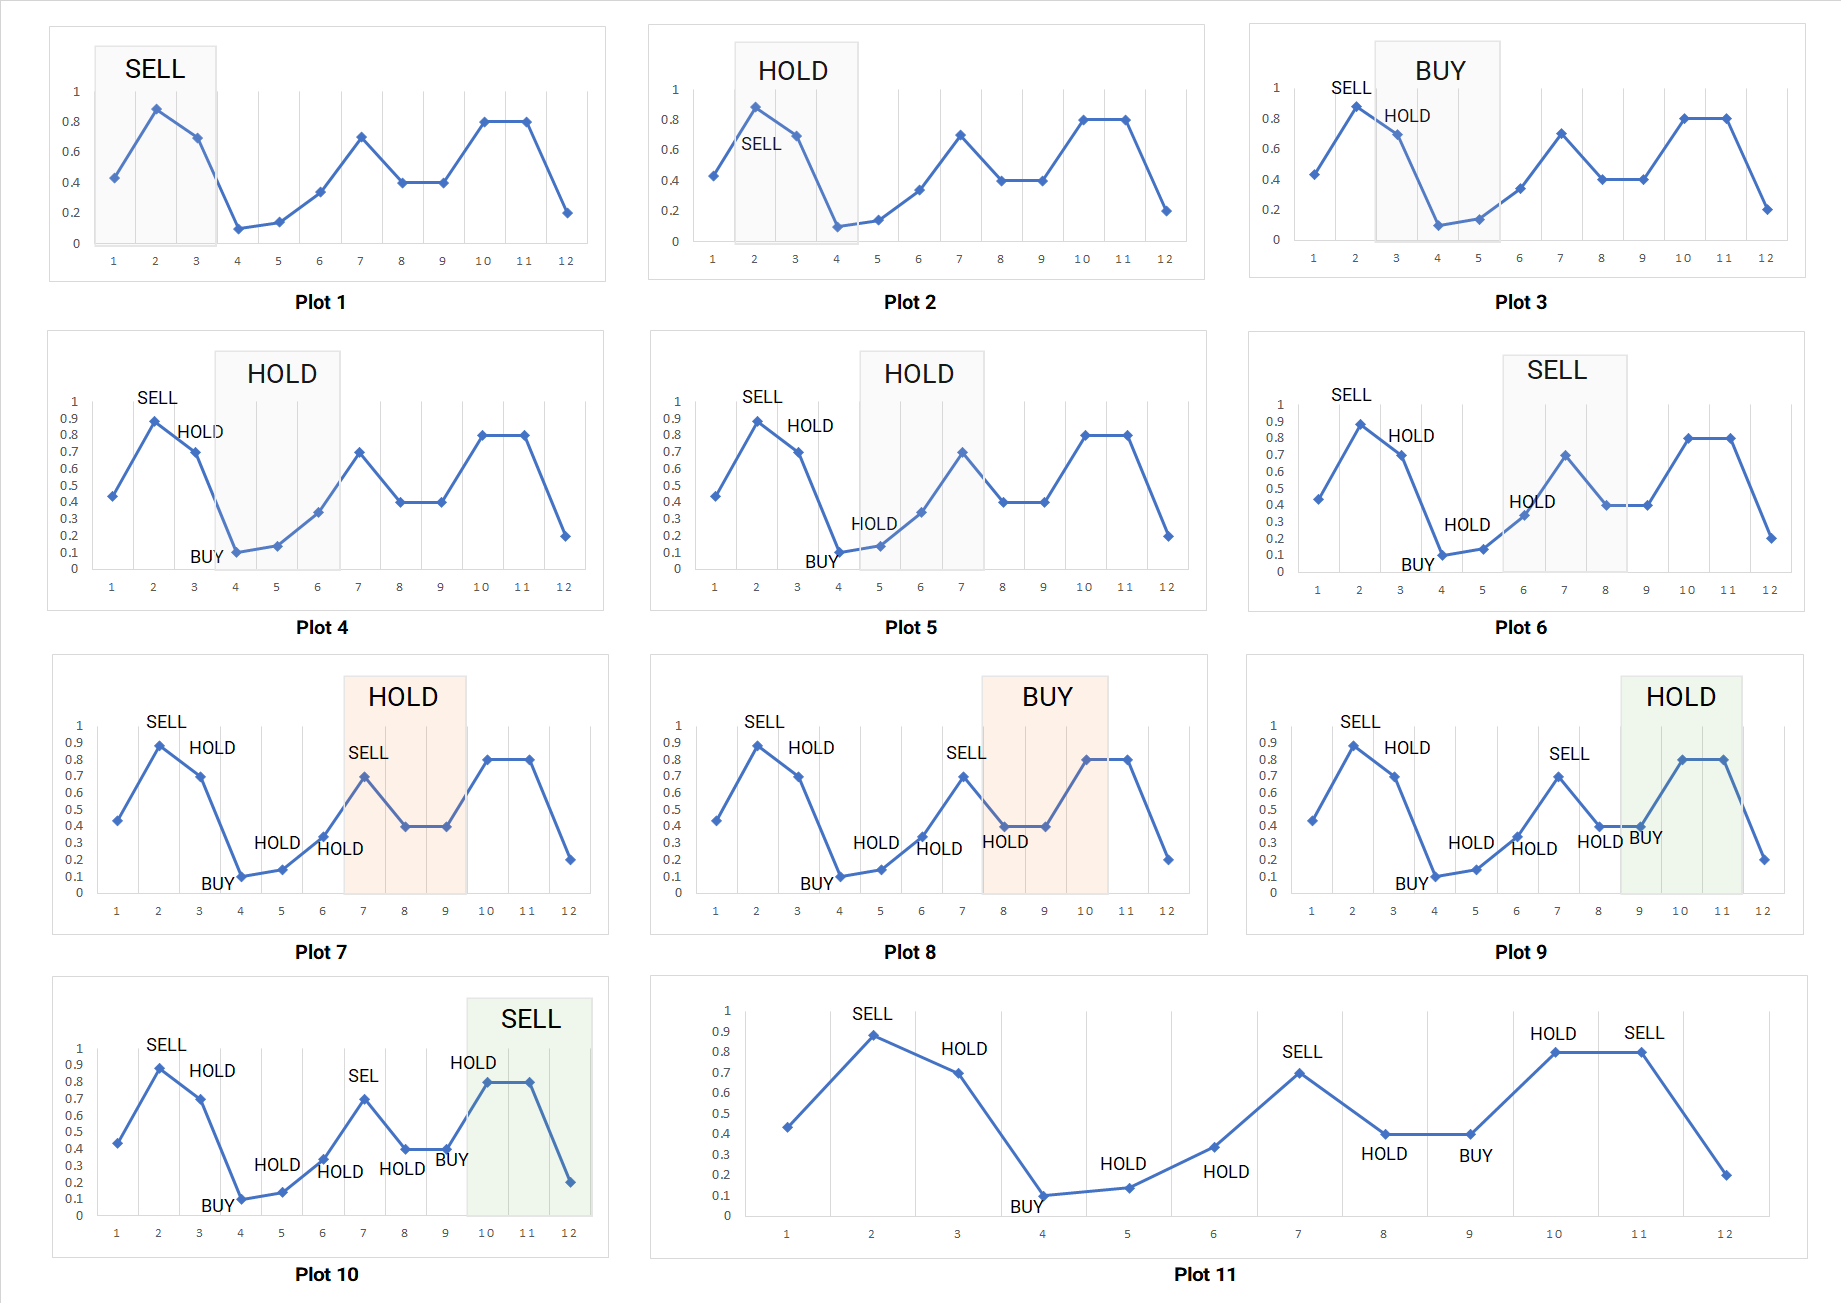
\includegraphics[width=\textwidth]{images/Labelling.png}
    \caption{Example of labelling. The figure visualizes the step-by-step labelling of an example series of $12$ observations with labelling window of size $l=3$. The grey rectangles show the scope of values considered in every labelling decision, and that the value in the middle time step is labelled in every step (Plots 1-6). Plots 7-8 show the process in the first special case, that is when the mid value is not the only local minimum, but shares this property with one of its neighbouring observations. The decision in the second special case, depicted in Plots 9-10, is similar, only with two consequent local maxima within the same window. It can also be seen in Plot 11 that the first and last $\lfloor \frac{l}{2} \rfloor = 1$ values cannot be labelled.}
    \label{fig:Labelling}
\end{figure}

\subsection{Recognizing Patterns with Deep CNN - NOT READY}
\label{subsec:DM:RecPatwCNN}
Deep convolutional neural networks (CNN) are artificial neural networks (ANN) with multiple layers between the input and output layers (deep) that also employ convolution in one or more layers as a substitute for the matrix multiplication (see p.326, Chapter 9 in \cite{goodfellow2016deep}). %As per Chapter 9.2 of \cite{goodfellow2016deep}) 
There are three main arguments why CNNs are relatively popular and some of these make them particularly advantageous for the model.
Firstly, it can process fairly raw high dimensional data and extract the most important features for the given exercise. Secondly, the sparse connectivity in the network prove to be computationally very efficient .... And last but not least, ...

textbf{Finish}

% Let us take a second to recap what we have so far. We have one-dimensional historical stock price data that we preprocessed and created images from the sliding windows of data points. We created 
%labels of trading actions on our original data and then matched these labels to the relevant images. 

SKELETON:

1. Feed image representations in different channels for colors

2. Optimize number of layers, neurons - maybe tiled CNN

3. Add regularization

5. Other additions/optimization

6. Description of exact build of each model

\subsection{Evaluation Techniques}

For assessing the technical performance of the CNN, we use accuracy, class-wise and average precision, recall and F1 scores, moreover we will also present the confusion matrix for the different models and testing periods. 
The confusion matrix allows us to observe the absolute number of correctly and wrongly classified observations by classes. 
\begin{figure}[ht]
    \centering
    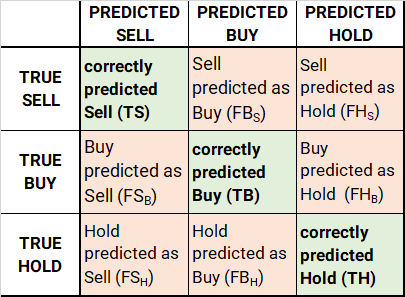
\includegraphics[width=.5\textwidth]{images/Confusion_matrix.png}
    \caption{The structure of the confusion matrix. The notations "TS", "TB", and "TH" mean True Sell, True Buy and True Hold, while "FS", "FB", and "FH" mean False Sell, Buy, and Hold, the subscript refers to the true class in case of false classification.}
    \label{fig:cmdef}
\end{figure}
The matrix that we will see in the section \nameref{subsec:ER:ClassPerf} has the structure described in Figure \ref{fig:cmdef}.
The accuracy tells us about the proportion of observations that is classified correctly over all the classes $k = \{S, B, H\}$ . Now, given we wish to calculate measurements for a classification on a set of $N$ values, i.e. $N = TS + TB + TH + \sum_k \left(FS_k + FB_k + FH_k\right)$ using the notations in Figure \ref{fig:cmdef}, the accuracy is:
\begin{equation}
    \label{eq:acc}
    Accuracy = \frac{TS + TB + TH}{N}
\end{equation}
the class-wise precision for each class $K$ is given by
\begin{equation}
    \label{eq:pr}
    Precision_K = \frac{TK}{TK +  \sum_k FK_k}
\end{equation}
and the class-wise recall is then 
\begin{equation}
    \label{eq:rec}
    Recall_K = \frac{TK}{TK +  \sum_{k  \smallsetminus \{K\}} Fk_K}
\end{equation}
or in other words, the precision of a class $K$ tells us the proportion of correct classifications among all the predictions of $K$, and the recall gives the percentage of the true $K$ class that is correctly classified as $K$. The F1 score is a useful measurement in unbalanced classification tasks, and it is the harmonic mean of the precision and the recall in every class:
\begin{equation}
    \label{eq:f1}
    F1_K = 2 \frac{Precision_K \cdot Recall_K}{Precision_K + Recall_K}.
\end{equation}
We will also see average results over the classes for each of these metrics.

Furthermore, financial assessment is carried out on the test data which we start by setting an initial capital of $C_0 = 10000$ and a flat transaction based trading commission of $c = 5$ (both in USD). At every time step $t$ the trading orders are executed as per the signals ($s_t$) at price $p_t$ which are predicted by the model for the respective time step.
In case of repeating consequent signals, the first signal prompts a trading action given cash/the asset is available in holdings. The Buy order is completed given money is available (up until the first Buy order, and after each executed Sell) and the Sell order is completed if units of the financial instrument are available for selling (i.e. after each executed Buy), otherwise they are handled as a Hold. In case of a Hold signal at $t$, trade does not take place, only the amount of capital $C_t$ is tracked at the given period.
Assets are assumed to be traded in any increments. Using the described approach over the period $t=1, \dots, T$ the following measurements are calculated for the financial performance evaluation:

\begin{itemize}
    \item number of all executed trades: $n_{trade}$
    \item total profit/loss: 
    \begin{align}
        \label{eq:totPL}
            P\& L = C_T - C_0
    \end{align}
    \item cumulative return: 
    \begin{align}
        \label{eq:cumret}
            r_c = \frac{P \& L}{C_0}
    \end{align}
    \item annualized return (for business year of 260 days): 
    \begin{align}
        \label{eq:annualized}
            r_{ann} = \frac{C_T}{C_0}^{\frac{260}{n}}-1
    \end{align}
    \item average P \& L per trade:
    \begin{align}
        \label{eq:avgpl}
        AvgP \& L = \frac{P \& L}{n_{trade}}
    \end{align}
\end{itemize}

To monitor the performance over different economic regimes, we test the model throughout 1 year periods in 2006, 2009 and May 2018 - June 2019. The models will be trained on all previous available data up to the first day of testing. 
Moreover, the evaluation of competing algorithmic trading techniques, for the same testing periods with the same financial metrics provided in Equations \ref{eq:totPL} - \ref{eq:avgpl}, are carried out to make the evaluation more comprehensive.
There are three methods considered for comparison: the Buy \& Hold, the momentum-based Relative Strength Index (RSI), and a volatility-based strategy using the Bollinger Bands (BB).\footnote{The strategies are described in the Appendices: \nameref{app:CompetingStrats}}

In order to assess feasibility we will also present how much time it takes for the model to train and to return predictions from the trained model.

\section{Evaluation Results}
\label{sec:ER}

\subsection{Classification Performance}
\label{subsec:ER:ClassPerf}
figures, confusion matrix, accuracy measurements, etc.

\subsection{Financial Performance}
\label{subsec:ER:FinPerf}
description of results of Financial Evaluation, tables, text

\subsection{Time Consumption}
\label{subsec:ER:TimePerf}
How long it takes to train, how long it takes to predict

\section{Discussion}
\label{sec:Discuss}

\section{Conclusion}
\label{sec:Conclusion}

\section{Appendices}
\label{sec:App}

\subsection{Gramian Angular Field: penalized inner product}
\label{app:GAF}
\begin{equation}
    \begin{split}
        \cos(\phi_1 + \phi_2)  & = \cos(\arccos(x) + \arccos(y)) \\
        & = \cos(\arccos(x)) \cdot \cos(\arccos(y)) - \sin(\arccos(x)) \cdot \sin(\arccos(y))\\
        & = x\cdot y - \sqrt{1-x^2} \cdot \sqrt{1-y^2}\\
        & = \langle x, y \rangle - \sqrt{1-x^2} \cdot \sqrt{1-y^2}
    \end{split}
\end{equation}
 Notice, that the entire operation does not satisfy the assumptions of an inner product (linearity limitation, not necessarily positive definite).

\subsection{Competing Strategies Description}
\label{app:CompetingStrats}

\subsubsection{Buy \& Hold}
The Buy \& Hold strategy is a simple and passive strategy based on buying an asset and keeping it for a long period of time, hoping for long term returns regardless of short term fluctuations on the market.
This will be represented in the testing periods as a Buy order on the first date and a Sell order on the last date with no other trades executed in between.

\subsubsection{Relative Strength Index}
The RSI (\cite{wilder1986relative}) is a momentum oscillator $[0, 100]$ with values over 70 indicating an overbought and below 30 and oversold asset. A Buy order happens when the RSI rises above 30 from below and a Sell is indicated by decreasing below 70 from above. The metric is defined by the two step calculation for a look-back period of $d=20$ days:
\begin{equation}
    \label{eq:RSI1}
    RSI_{step1} = 100 - \left[ \frac{100}{1 + \frac{Avg_d Gain}{Avg_d Loss}}\right]
\end{equation}
where $Avg_d Gain$ and $Avg_d Loss$ are the average percentage gains and/or losses during a look-back period of length $d$. After the first $d$ periods of data is available, the second step is just the smoothing of the step 1 formula:
\begin{equation}
    \label{eq:RSI2}
    RSI_{step2} = 100 - \left[ \frac{100}{1 + \frac{Previous Avg_d Gain \cdot (d-1) + Current Gain}{Previous Avg_d Loss \cdot (d-1) + Current Loss}}\right].
\end{equation}

\subsubsection{Bollinger Bands}
The Bollinger Bands (BB) (\cite{bollinger2002bollinger}) characterize the prices and the volatility of a financial asset. They can be depicted on the chart of an asset as a graphical band showing the envelope maximum and minimum of moving averages over the look- back period $d=20$, and the volatility is represented by the width of the envelope.
If the $d$-period moving average is given by $MA_d$, the $d$-period standard deviation is given by $\sigma_d$ and $c=2$ is a customizable parameter then the bands are:
\begin{equation}
    \label{eq:BBlow}
    lowerBB = MA_d - c \sigma_d
\end{equation}
and
\begin{equation}
    \label{eq:BBup}
    upperBB = MA_d + c \sigma_d.
\end{equation}
The strategy is to Buy when the Adjusted Close price decreases below the $lowerBB$ and Sell if it increases above the $upperBB$.

\bibliography{reference}
\bibliographystyle{apalike}

\end{document}
